\apendice{Especificación de diseño}

\section{Introducción}

En este apéndice vamos a tratar de todo aquello relacionado a la organización del proyecto.

\section{Diseño de datos}

A lo largo de este proyecto la cantidad de datos con la que hemos trabajado es muy grande, dada la necesidad de datos de una red neuronal para un buen pronóstico. En la sección vamos a ver como hemos almacenado estos datos y que uso hemos hecho de estos.

\subsection{Almacenamiento de datos}

Los datos han sido almacenados en el sistema de gestión de bases de datos relacionales MySQL, esta  la hemos administrado utilizando PHPMyAdmin. Dada la gran cantidad de datos y su diversidad ha sido necesario trabajar con diferentes tablas, como podemos observar en el modelo relacional \ref{fig:ModRel}, aquí podemos observar todas las tablas y sus relaciones con la excepción de la tabla de partidos, que podemos observar en esta figura \ref{fig:ModRelPar}, dado que esta posee una enorme cantidad de campos.

Como se puede observar en el modelo relacional la tabla \textit{balance\_general} se encuentra apartada del resto, y es que esta tabla ha sido creada para evitar tener que hacer todos los cálculos de cada jornada al cargar la ventana \textit{Informe general}.

\begin{figure}
\centering
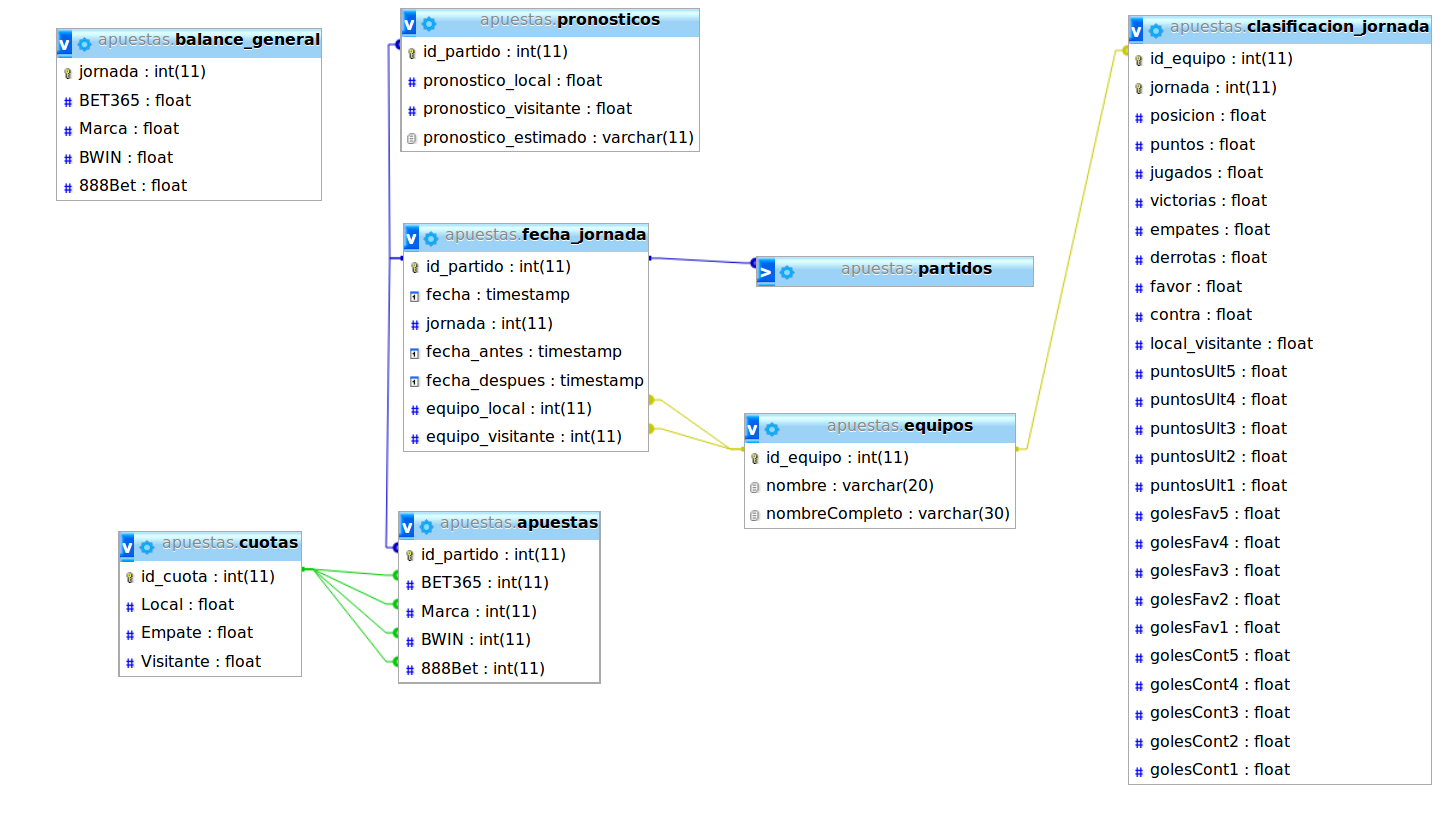
\includegraphics[width=.9\textwidth]{img/modelo_relacional}
\caption{Modelo relacional}
\label{fig:ModRel}
\end{figure}

\begin{figure}
\centering
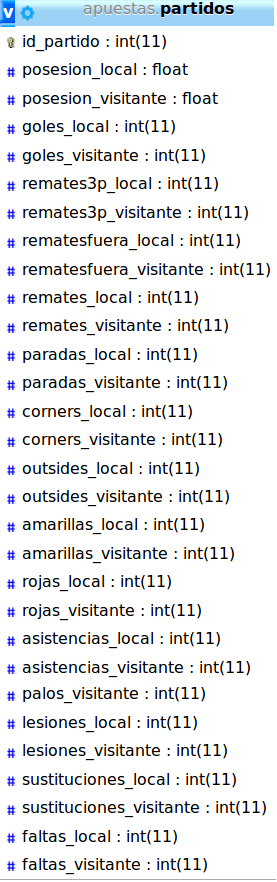
\includegraphics[width=.5\textwidth]{img/modelo_relacional_partidos}
\caption{Tabla de partidos}
\label{fig:ModRelPar}
\end{figure}

A continuación se van a explicar cada una de las tablas utilizadas:

\begin{itemize}
\item \textbf{equipos} En esta tabla encontramos los 20 equipos de primera división, se han dispuesto alfabéticamente y esta tabla posee tres campos, entre ellos está el nombre, este campo es muy importante a la hora de realizar el scraing, ya que es así como identifica la web a cada equipo, el tercer y último campo es <<nombreCompleto>>, utilizado para mostrar el nombre de dicho equipo en la interfaz.

\item \textbf{fecha\_jornada}Esta tabla contiene cada partido de cada jornada de la liga, con algunos campos como la fecha, la jornada o los equipos contendientes.

\item \textbf{clasificacion\_jornada} Aquí podemos observar la posición en la clasificación de cada uno de los equipos en cada jornada, así comolas últimas rachas de los equipos. Esta tabla resulta fundamental a la hora de insertar datos en la red neuronal.

\item \textbf{partidos} Mediante las técnicas de scraping extraemos datos de cada partido, estos datos son almacenados aquí y contiene todas las estadísticas de ambos equipos. Los datos son utilizados para la entrada en la red neuronal.

\item \textbf{pronosticos} Esta tabla contiene la salida de datos de la red neuronal y el resultado final obtenido por esta para cada uno de lo partidos.

\item \textbf{apuestas} Organiza todas las cuotas de las casas de apuestas para cada partido, registrando todos los identificadores.

\item \textbf{cuotas} Posee las cuotas y sus valores dependiendo de la victoria local, empate o victoria visitante.

\item \textbf{balance\_general} Almacena el balance de cada casa de apuestas en cada jornada, esta tabla se utiliza posteriormente para mostrarla en la interfaz.
\end{itemize}
\section{Diseño procedimental}
En esta sección se va a poder observar el funcionamiento del proyecto.

\subsection{Diagrama de flujo}
En esta imagen \ref{fig:DiagFluj} podemos ver la ejecución del programa y de su dependencia del día en el que nos encontremos. Los campos \textit{fecha\_antes} y \textit{fecha\_despues} son el día previo y posterior a una jornada. Usualmente es trata del viernes a las 00:00 y  de Martes a las 00:00, esto es así por que el primer partido de la jornada suele disputarse el viernes a las 20:45 y el último el lunes a las 20:45.

Una vez ejecutados los algoritmos de backpropagation y del scraping de casas de apuestas, el usuario ya podrá acceder al informe pronóstico donde gozará de toda la información disponible.

En cuanto se ejecutan los algoritmos de scraping de resultados y clasificación y cálculo de rachas, el usuario ya podrá acceder sin problemas a la información actualizada de como ha ido la jornada, ya que se actualizará la ventana de informe de jornada y a su vez el informe global.
\begin{figure}
\centering
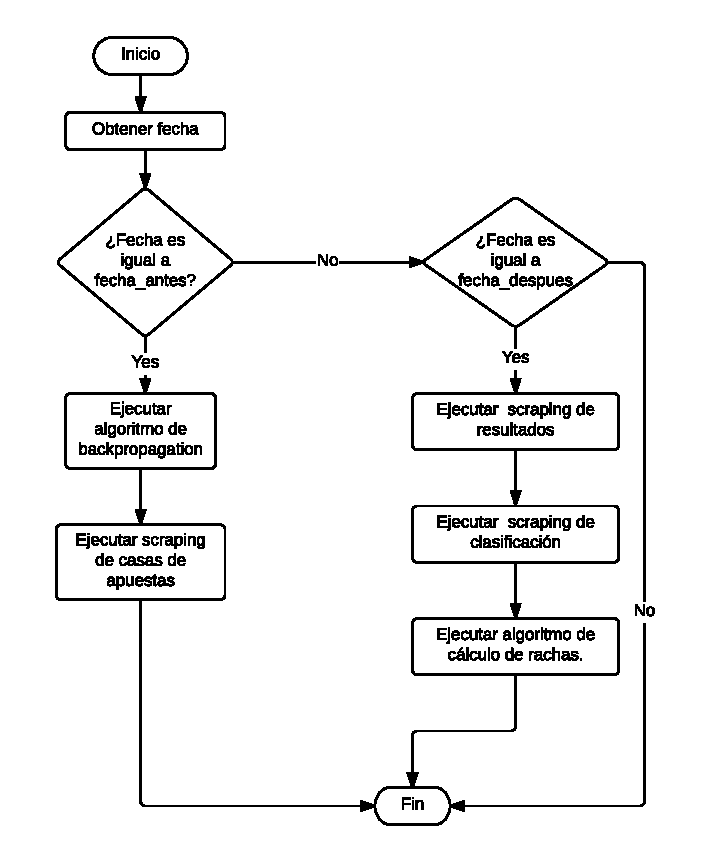
\includegraphics[width=.9\textwidth]{img/diagrama_flujo}
\caption{Diagrama de flujo}
\label{fig:DiagFluj}
\end{figure}

\section{Diseño arquitectónico}
Se ha utilizado una arquitectura cliente servidor, esta consiste en un cliente que realiza peticiones a otro <<servidor>> el cual le proporciona la respuesta. Actualmente esta es la forma de trabajo más extendida en la comunicación por redes.

El servidor espera solicitudes en un puerto, el cliente es quien realiza estas solicitudes, a su vez el cliente reserva un puerto desde el cual realizar las solicitudes. Utilizando esta arquitectura el cliente tiene la libertad de obtener la información que desea cuando quiera y de diferentes origenes.\cite{cliente_servidor}

El modelo utilizado en este proyecto ha sido el de tres niveles, similar al que podemos observar en esta figura\ref{fig:CliSer}, incluimos una base de datos donde incluye y extrae datos el servidor. Nuestro servidor es un Apache y  la base de datos elegida es MySQL. En la arquitectura de tres niveles, las aplicaciones a nivel de servidor son descentralizadas, permitiendo un mayor grado de flexibilidad, mayor seguridad y mejor rendimiento.

\begin{figure}
\centering
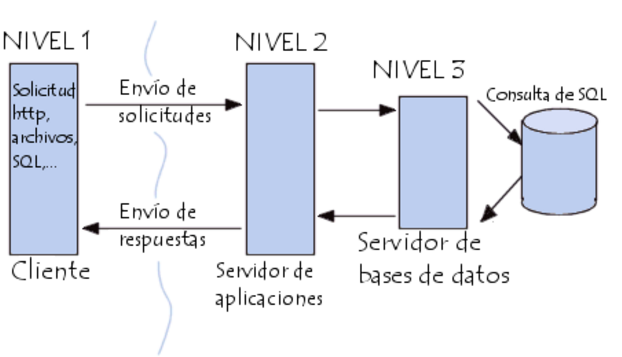
\includegraphics[width=.9\textwidth]{img/cliente_servidor}
\caption{Arquitectura de tres niveles Cliente servidor}
\label{fig:CliSer}
\end{figure}



